
\section{All results}
\label{appendix:all-results}

% Commented out because it fails to compile ATM
% Dataset 1
\subsection{Dataset 1 - Experiment results}
\import{./tables/results/dataset_1}{sarima-dataset-1.tex}

\import{./tables/results/dataset_1}{local-univariate-lstm-dataset-1.tex}
\import{./tables/results/dataset_1}{global-univariate-lstm-dataset-1.tex}
\import{./tables/results/dataset_1}{local-multivariate-lstm-dataset-1.tex}
\import{./tables/results/dataset_1}{global-multivariate-lstm-dataset-1.tex}


\import{./tables/results/dataset_1}{local-univariate-cnn-ae-lstm-dataset-1.tex}
\import{./tables/results/dataset_1}{global-univariate-cnn-ae-lstm-dataset-1.tex}
\import{./tables/results/dataset_1}{local-multivariate-cnn-ae-lstm-dataset-1.tex}
\import{./tables/results/dataset_1}{global-multivariate-cnn-ae-lstm-dataset-1.tex}


% Dataset 2
\subsection{Dataset 2 - Experiment results}
\import{./tables/results/dataset_2}{sarima-dataset-2.tex}

\import{./tables/results/dataset_2}{local-univariate-lstm-dataset-2.tex}
\import{./tables/results/dataset_2}{global-univariate-lstm-dataset-2.tex}
\import{./tables/results/dataset_2}{local-multivariate-lstm-dataset-2.tex}
\import{./tables/results/dataset_2}{global-multivariate-lstm-dataset-2.tex}

\import{./tables/results/dataset_2}{local-univariate-cnn-ae-lstm-dataset-2.tex}
\import{./tables/results/dataset_2}{global-univariate-cnn-ae-lstm-dataset-2.tex}
\import{./tables/results/dataset_2}{local-multivariate-cnn-ae-lstm-dataset-2.tex}
\import{./tables/results/dataset_2}{global-multivariate-cnn-ae-lstm-dataset-2.tex}

% Dataset Seasonal
\subsection{Dataset 3 - Experiment results}
\import{./tables/results/dataset_seasonal}{sarima-dataset-3.tex}

\import{./tables/results/dataset_seasonal}{local-univariate-lstm-dataset-3.tex}
\import{./tables/results/dataset_seasonal}{global-univariate-lstm-dataset-3.tex}
\import{./tables/results/dataset_seasonal}{local-multivariate-lstm-dataset-3.tex}
\import{./tables/results/dataset_seasonal}{global-multivariate-lstm-dataset-3.tex}

\import{./tables/results/dataset_seasonal}{local-univariate-cnn-ae-lstm-dataset-3.tex}
\import{./tables/results/dataset_seasonal}{global-univariate-cnn-ae-lstm-dataset-3.tex}
\import{./tables/results/dataset_seasonal}{local-multivariate-cnn-ae-lstm-dataset-3.tex}
\import{./tables/results/dataset_seasonal}{global-multivariate-cnn-ae-lstm-dataset-3.tex}

% Additional experiments -> Variance
\subsection{Dataset with variance - Additional Experiments}
\import{./tables/results/dataset_variance}{dataset-high-variance-cnn-ae-lstm-local-univariate-dataset-variance.tex}
\import{./tables/results/dataset_variance}{dataset-high-variance-lstm-local-univariate-dataset-variance.tex}
\import{./tables/results/dataset_variance}{low-variance-cnn-ae-lstm-local-univariate-dataset-variance.tex}
\import{./tables/results/dataset_variance}{low-variance-cnn-ae-lstm-local-univariate-dataset-variance.tex}
\import{./tables/results/dataset_variance}{ok-variance-lstm-local-univariate-dataset-variance.tex}
\import{./tables/results/dataset_variance}{ok-variance-lstm-local-univariate-dataset-variance.tex}

% Additional experiments -> Differencing
\subsection{Dataset with differencing - Additional Experiments}
\import{./tables/results/dataset_diff}{local-univariate-lstm-dataset-1-dataset-diff.tex}
\import{./tables/results/dataset_diff}{local-univariate-lstm-dataset-1-diff-dataset-diff.tex}
\import{./tables/results/dataset_diff}{local-univariate-lstm-dataset-3-dataset-diff.tex}
\import{./tables/results/dataset_diff}{local-univariate-lstm-dataset-3-diff-dataset-diff.tex}


% T-test values
\subsection{T-test statistical significance test results}
\import{./tables/results/ttest}{ttest-p-values-differencing-experiments-MASE.tex}
\import{./tables/results/ttest}{ttest-p-values-lstm-experiments-MASE-all-datasets.tex}
\import{./tables/results/ttest}{ttest-p-values-lstm-experiments-MASE-dataset-1.tex}
\import{./tables/results/ttest}{ttest-p-values-lstm-experiments-MASE-dataset-2.tex}
\import{./tables/results/ttest}{ttest-p-values-lstm-experiments-MASE-dataset-3.tex}
\import{./tables/results/ttest}{ttest-p-values-lstm-experiments-sMAPE-dataset-1.tex}
\import{./tables/results/ttest}{ttest-p-values-lstm-experiments-sMAPE-dataset-2.tex}
\import{./tables/results/ttest}{ttest-p-values-lstm-experiments-sMAPE-dataset-3.tex}
\import{./tables/results/ttest}{ttest-p-values-lstm-experiments-MASE.tex}
\import{./tables/results/ttest}{ttest-p-values-lstm-experiments-sMAPE.tex}
\import{./tables/results/ttest}{ttest-p-values-lstm-experiments-sMAPE-all-dataset.tex}
\import{./tables/results/ttest}{ttest-p-values-main-experiments-MASE.tex}

% Figures

\begin{figure}
  \centering
  \caption{Test predictions for local univariate LSTM on category 11850 with last week values ploted as a reference.}
  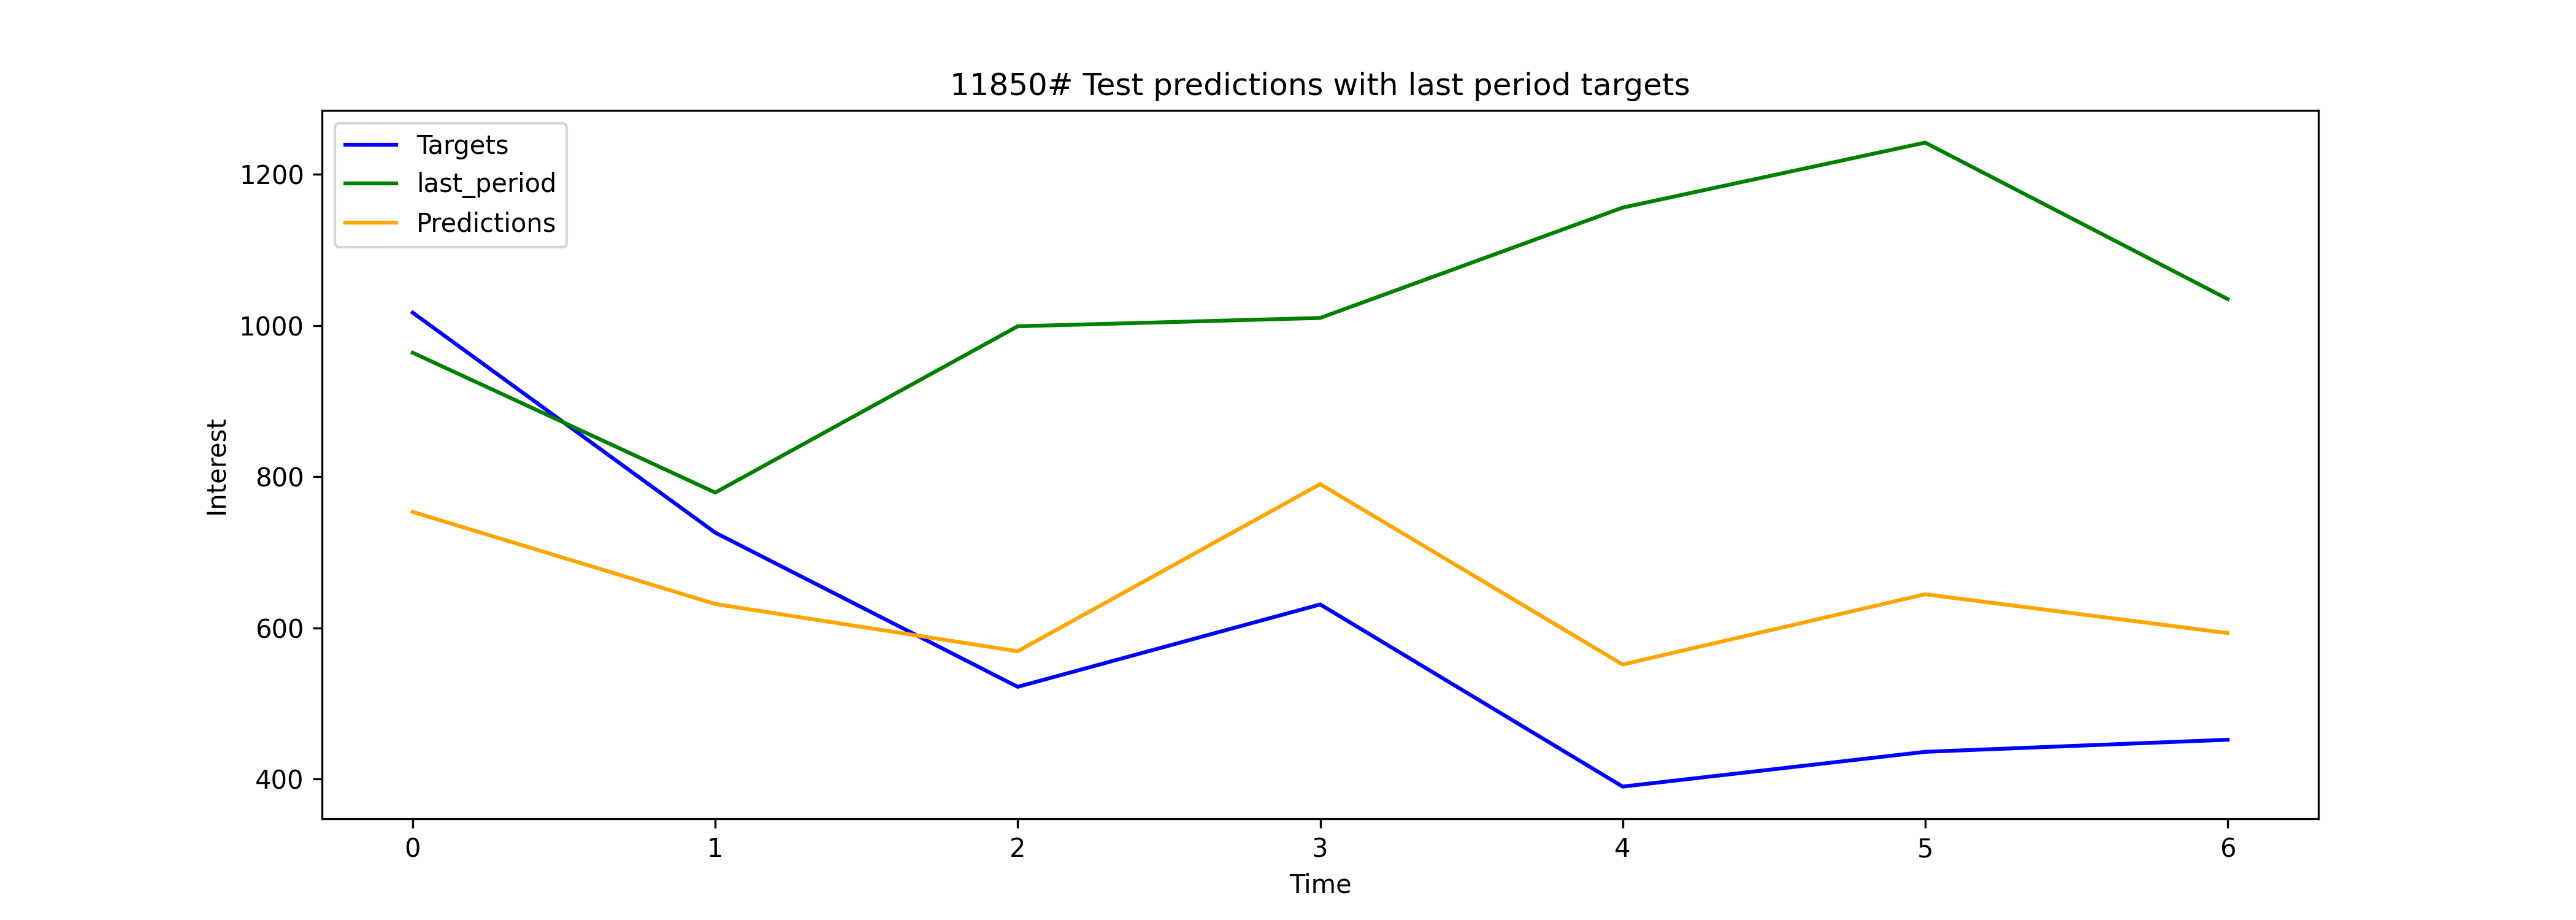
\includegraphics[width=\textwidth]{./figs/results/predictions/11850_Test_predictions_with_last_period_targets.png}
  \hfill
  \label{fig:results:predictions:11850-Test_predictions_with_last_period_targets.png}
\end{figure}

\begin{figure}
  \centering
  \caption{Test predictions for local univariate LSTM on category 12322 with last week values ploted as a context.}
  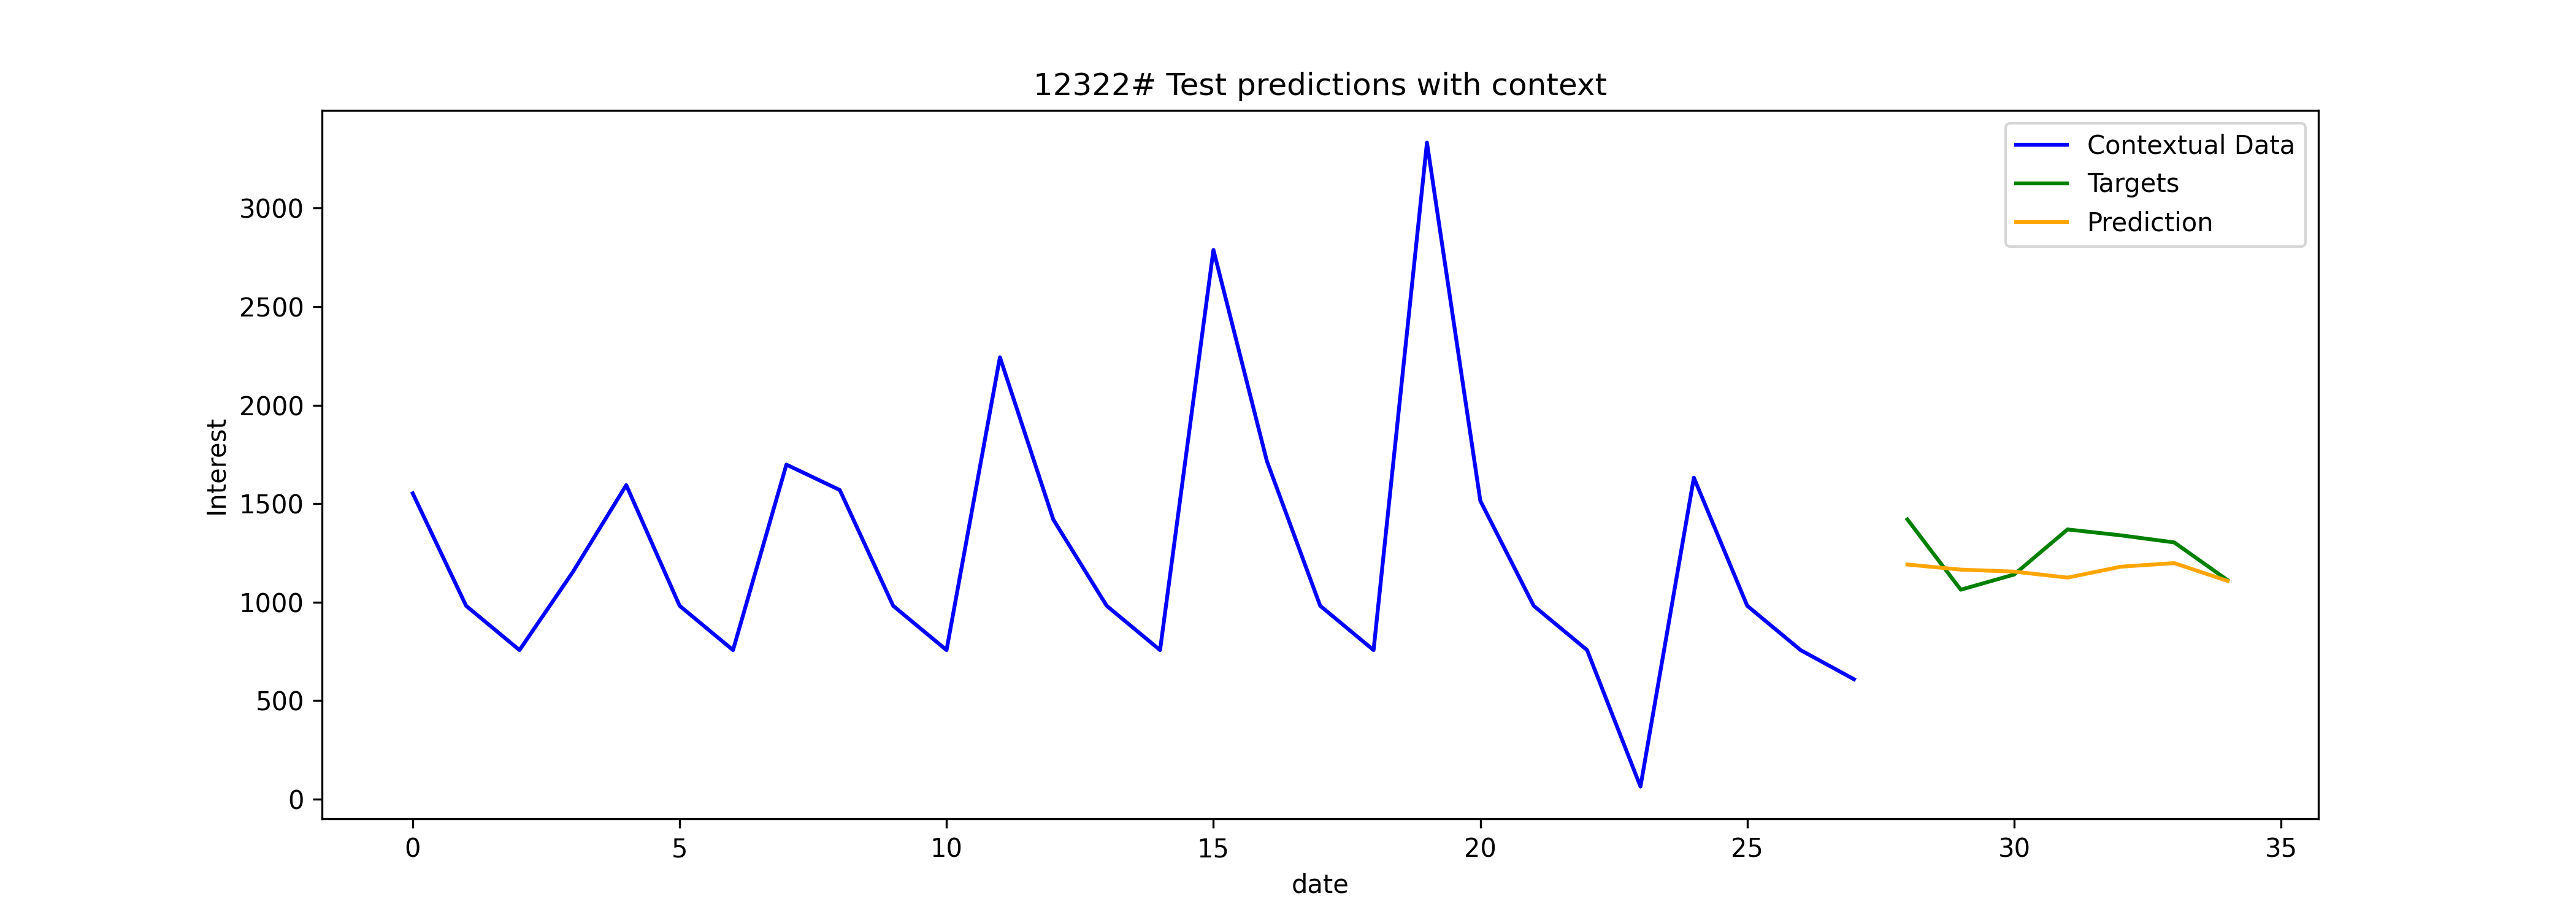
\includegraphics[width=\textwidth]{./figs/results/predictions/12322_Test_predictions_with_context.png}
  \hfill
  \label{fig:results:predictions:12322-Test_predictions_with_last_period_context.png}
\end{figure}

% TODO: Få til å legge inn de siste!
% \begin{figure}
%   \centering
%   \caption{Convolutional Autoencoders output to the LSTM on the test set from category 22}
%   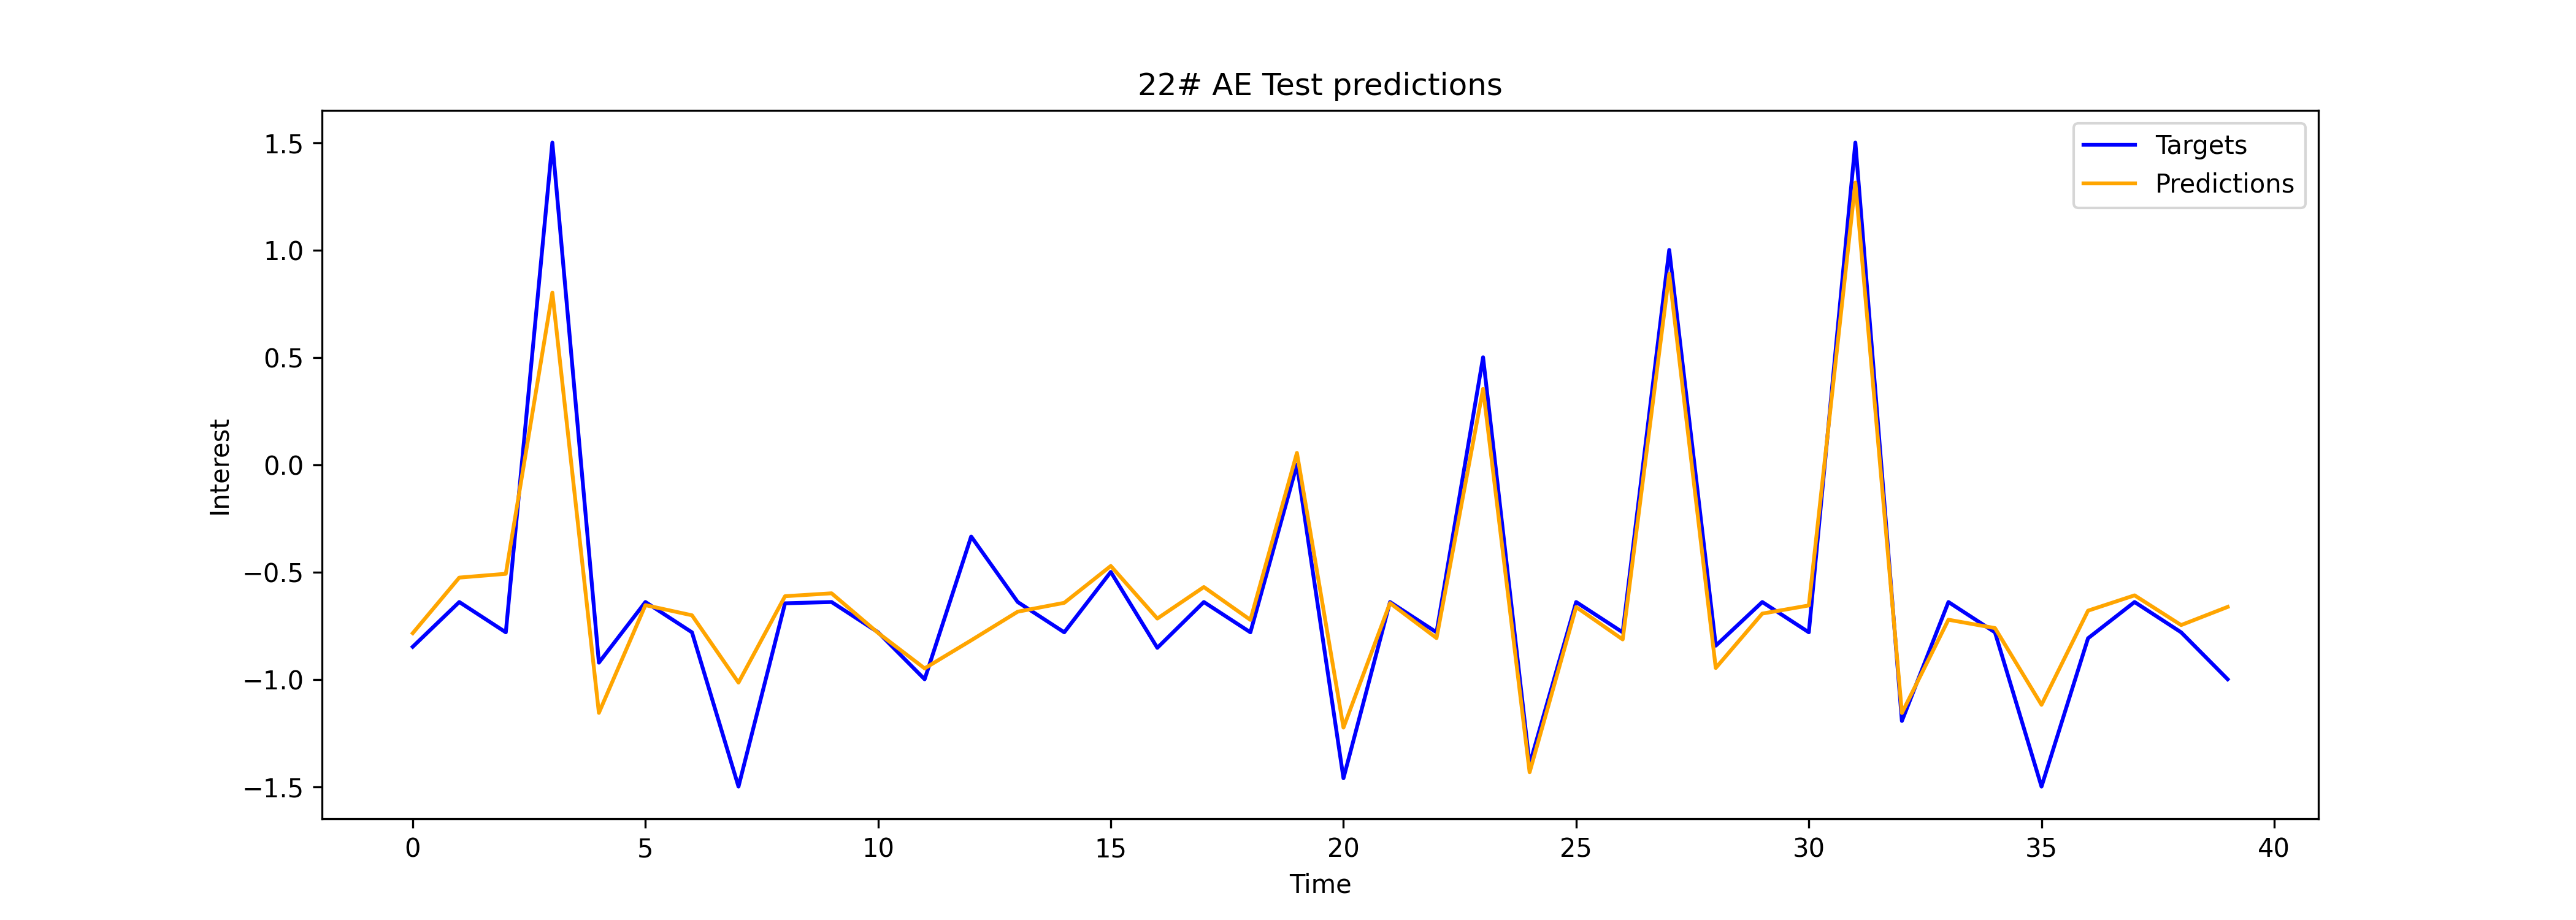
\includegraphics[width=0.7\textwidth]{./figs/results/predictions/22_AE_Test_predictions.png}
%   \hfill
%   \label{fig:results:predictions:22_AE_Test_predictions}
% \end{figure}


% \begin{figure}
%   \centering
%   \caption{Global univariate LSTM training predictions on the concatonated training set}
%   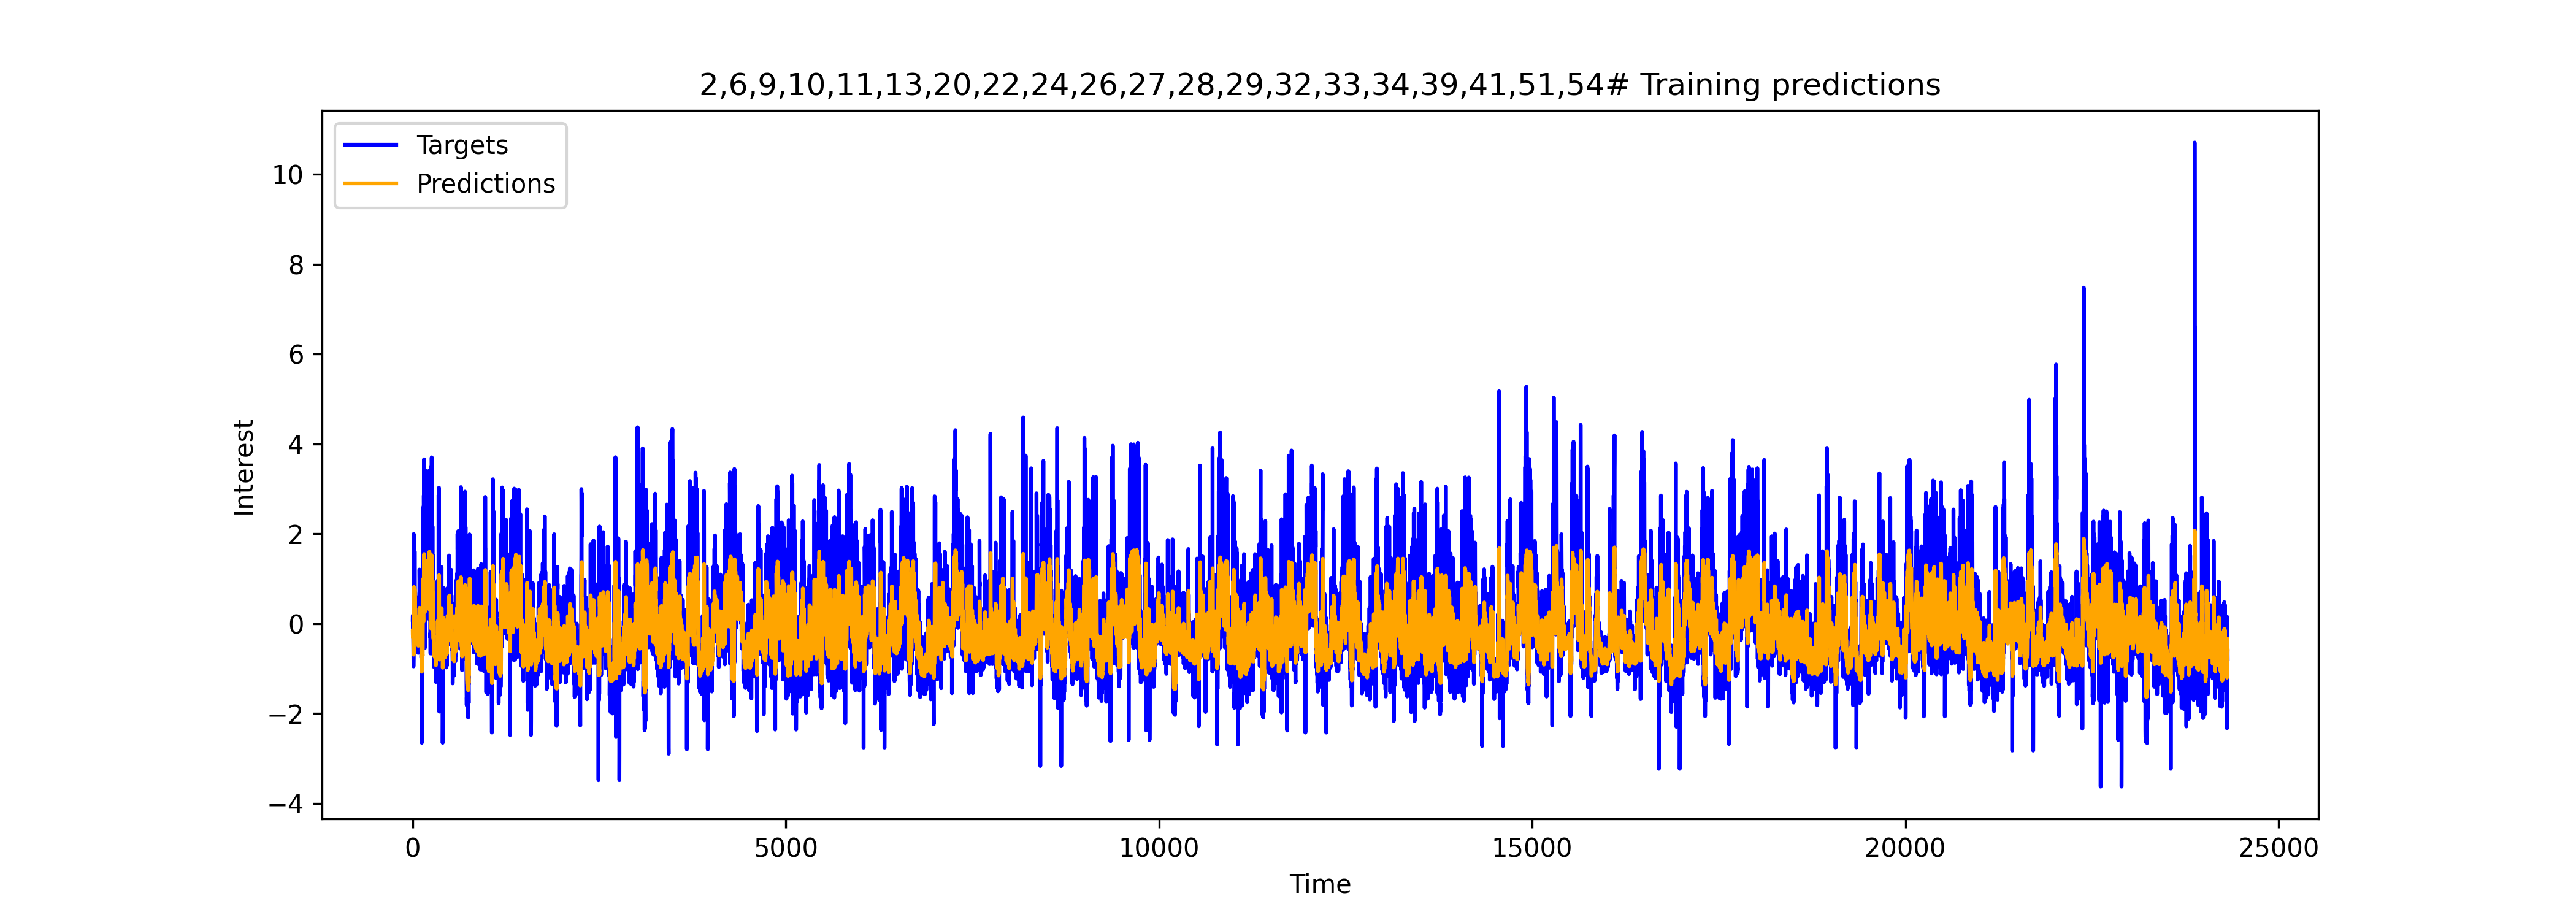
\includegraphics[width=0.7\textwidth]{./figs/results/predictions/2,6,9,10,11,13,20,22,24,26,27,28,29,32,33,34,39,41,51,54_Training_predictions.png}
%   \hfill
%   \label{fig:results:predictions:2,6,9,10,11,13,20,22,24,26,27,28,29,32,33,34,39,41,51,54_Training_predictions}
% \end{figure}
